\documentclass[a4paper,10pt]{article}

\usepackage[english]{babel}
\usepackage[utf8]{inputenc}
\usepackage{graphicx}
\usepackage{amsmath,amssymb}
\usepackage{subcaption}
\usepackage{hyperref, url}
 \usepackage[table,xcdraw]{xcolor}
\parindent 0mm
\parskip 3mm

% add your name and student number in parenthesis
\title{Survival Analysis of TCGA dataset}
\author{ Sailendra Pradhananga (sailendra.pradhanaga@scilifelab.se)\\ \\
			Project Report:Algorithms in Bioinformatics}

\begin{document}

\maketitle

\section{Introduction}


Survival analysis are statistical toolkits that are used to analyzing the outcome of variables based on time period of event occurrence. The event could be either be death, outbreak of disease or failure of automobile parts which are then followed specified time period in days, weeks or years. The major part of the these type of data involves two kinds of variables: first is the time to event and second whether the event have occurred or not. Based on different methods such as non parametric model such Kaplan Meier method or regression model such as cox proportional hazards two function, survival function and hazard function. The survival function gives the probability  for each time-points of surviving up to that events while hazard function whether the event has occurred or not  given the individual has survived or not. The main aim of these type of analysis is find the relationship between the survival time and variables under study such as drugs, gene expression, treatment  either with different covariates such as age, gender, race.

In the current project, we are provided a liver cancer patients of different races  dataset survival time and gene expression dataset of various grades. The main aim was to model the data with survival model in order find the potential prognostic marker for survival of patients using Cox Proportional Hazard models. Additionally, using the multiple hypothesis correction we predicted 4698 gene transcripts at 0.05 FDR. 

\section{Method}

	\subsection{TCGA Dataset}
The  TCGA dataset for the analysis was download from the (http://kaell.org/files/survivalLIHC.txt) site. As already stated in the project guidelines, these are the cancer patient expression data from the sequenced liver tumor.  Additionally there are few other features implication each cancer patient ethnicity, sex and cancer types.  These data were first read into python notebook as pandas dataframe  as done in  jupyter notebook.  Additional exploratory analysis was done in the notebook itself. The  dataset consists of both categorical features and numerical data of gene expression dataset. 

	\subsection {Preprocessing of Dataset}
In the survival analysis, the different categorical features were provided of liver cancer patients. These categorical features includes Gender, Race, Stage , Status, Age and LivingDays of different cancer patients.  These categorical features were then coded into different numerical codes . Originally, the dataset consists of gene expression profile os $19,571$. Furthermore, only those gene expression data were taken which had at least an expression in one of the patients.  

	\subsection{Cox proportional Hazard model}
	 Cox proportional hazards regression, used to relate several risk factors or exposures, considered simultaneously, to survival time. In the current project we used the implementation of Cox regression hazard model implemented on lifelines packages. Although I had tried including other covariates such as age and temperature to be used in the model, at this phase we have used indivudal expression of each gene transcript iteratively in order to get hazard function and survival rates of each gene transcripts. 
	 
	\subsection {Multiple testing correction}
	As discussed in earlier exercises we have  implemented mutliple testing correction for all the p.value estimates of gene expression for liver cancer to occur. However since we are testing multiple features, the pvalue $<$ 0.05 might be too lenient estimates. Hence based on storey and tribasni papser \cite {} an q value estimates were made of all the pvalues calcualted.
	 


 \section{Result}
 
 	\subsection {TCGA Liver cancer charcterstics}
 
 The data consists of 6 categorical features as shown in table 1 . Additionally since we are interested to know the dependent variable of event that in our case alive and death as a function of Living day we can observe the marked difference of alive and death events in patient cohort .  Additionally, there is markedly difference in gender distribution  in cancer cohort with more than half of the patient are male as shown in fig 2  and table 1

\begin{figure}[bh]
    \centering
      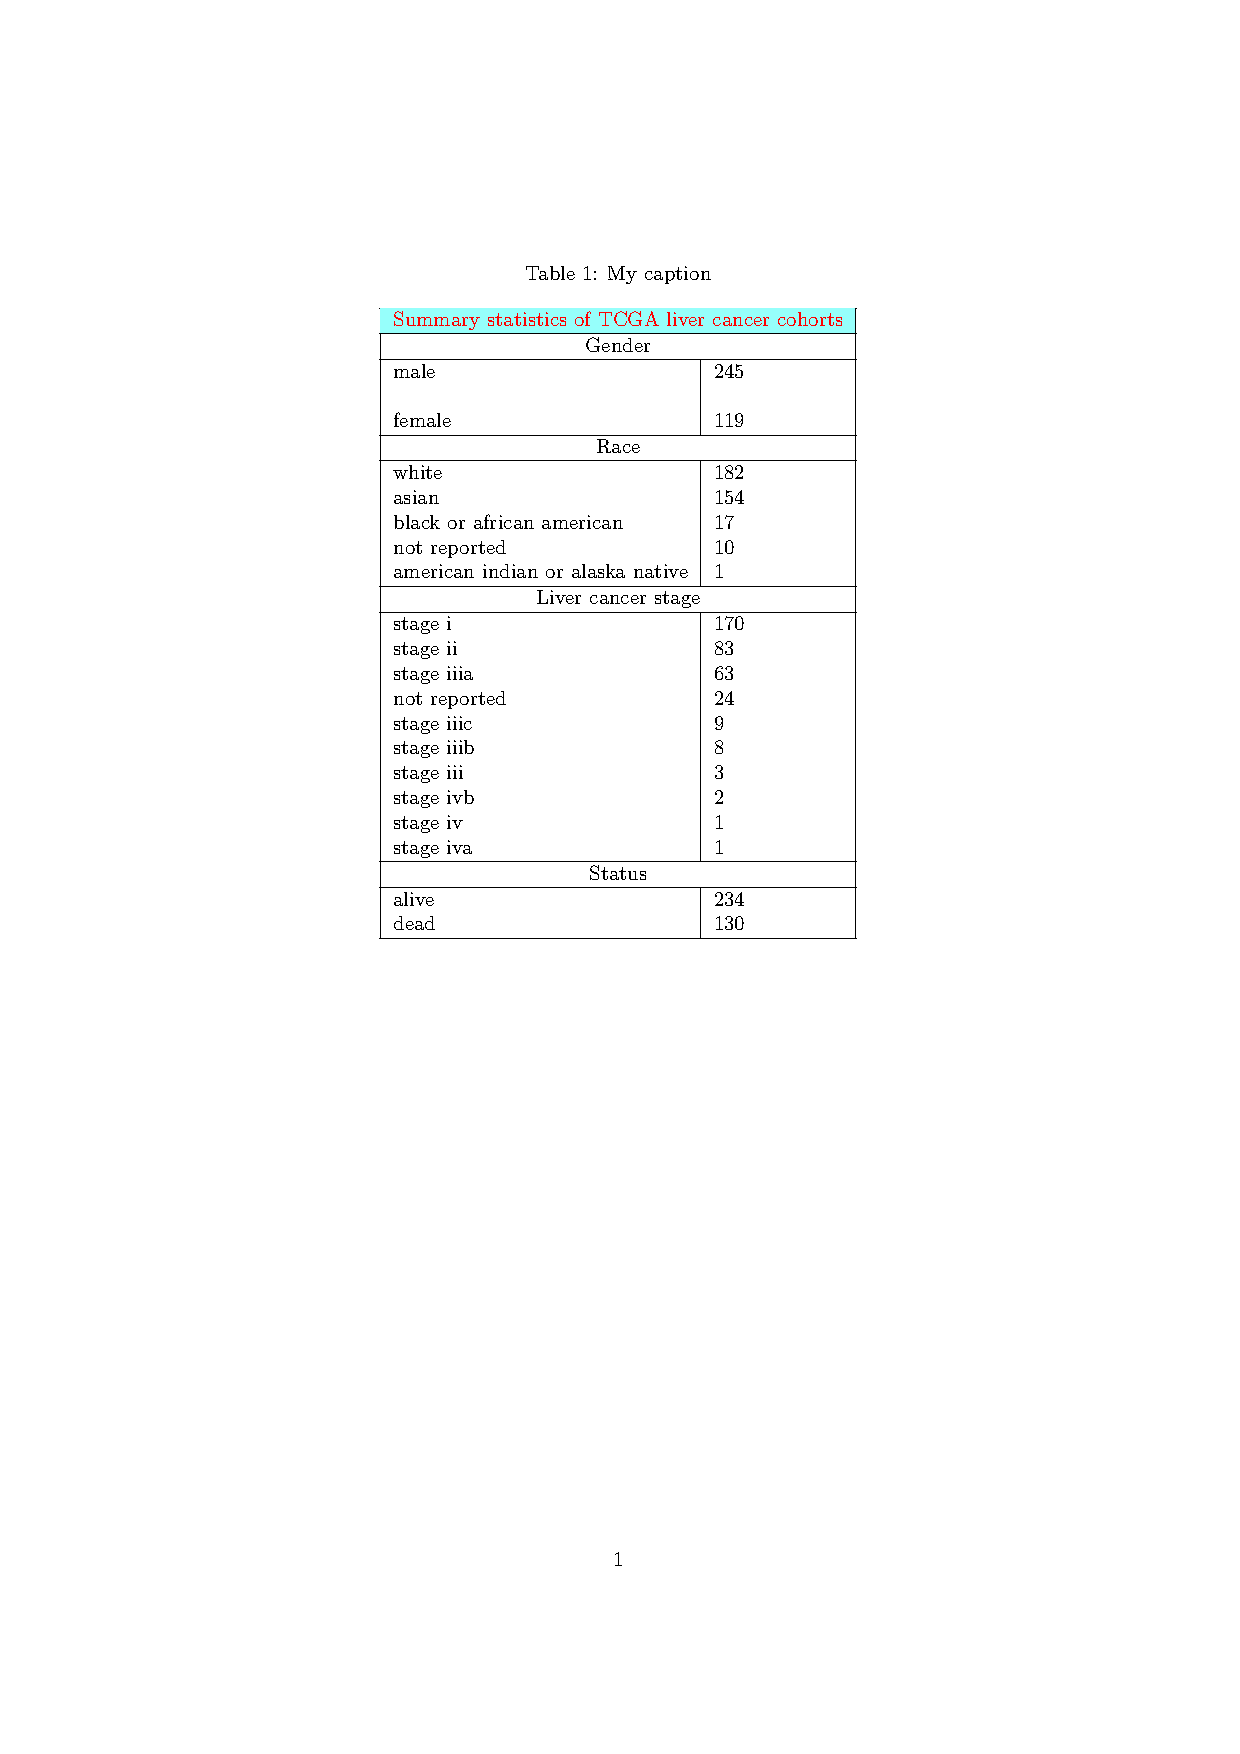
\includegraphics[width=\textwidth]{table.pdf}
    \caption{Pictures of animals}\label{fig:animals}
\end{figure}
  

\begin{figure}[bh]
    \centering
    \begin{subfigure}[h]{0.45\textwidth}
        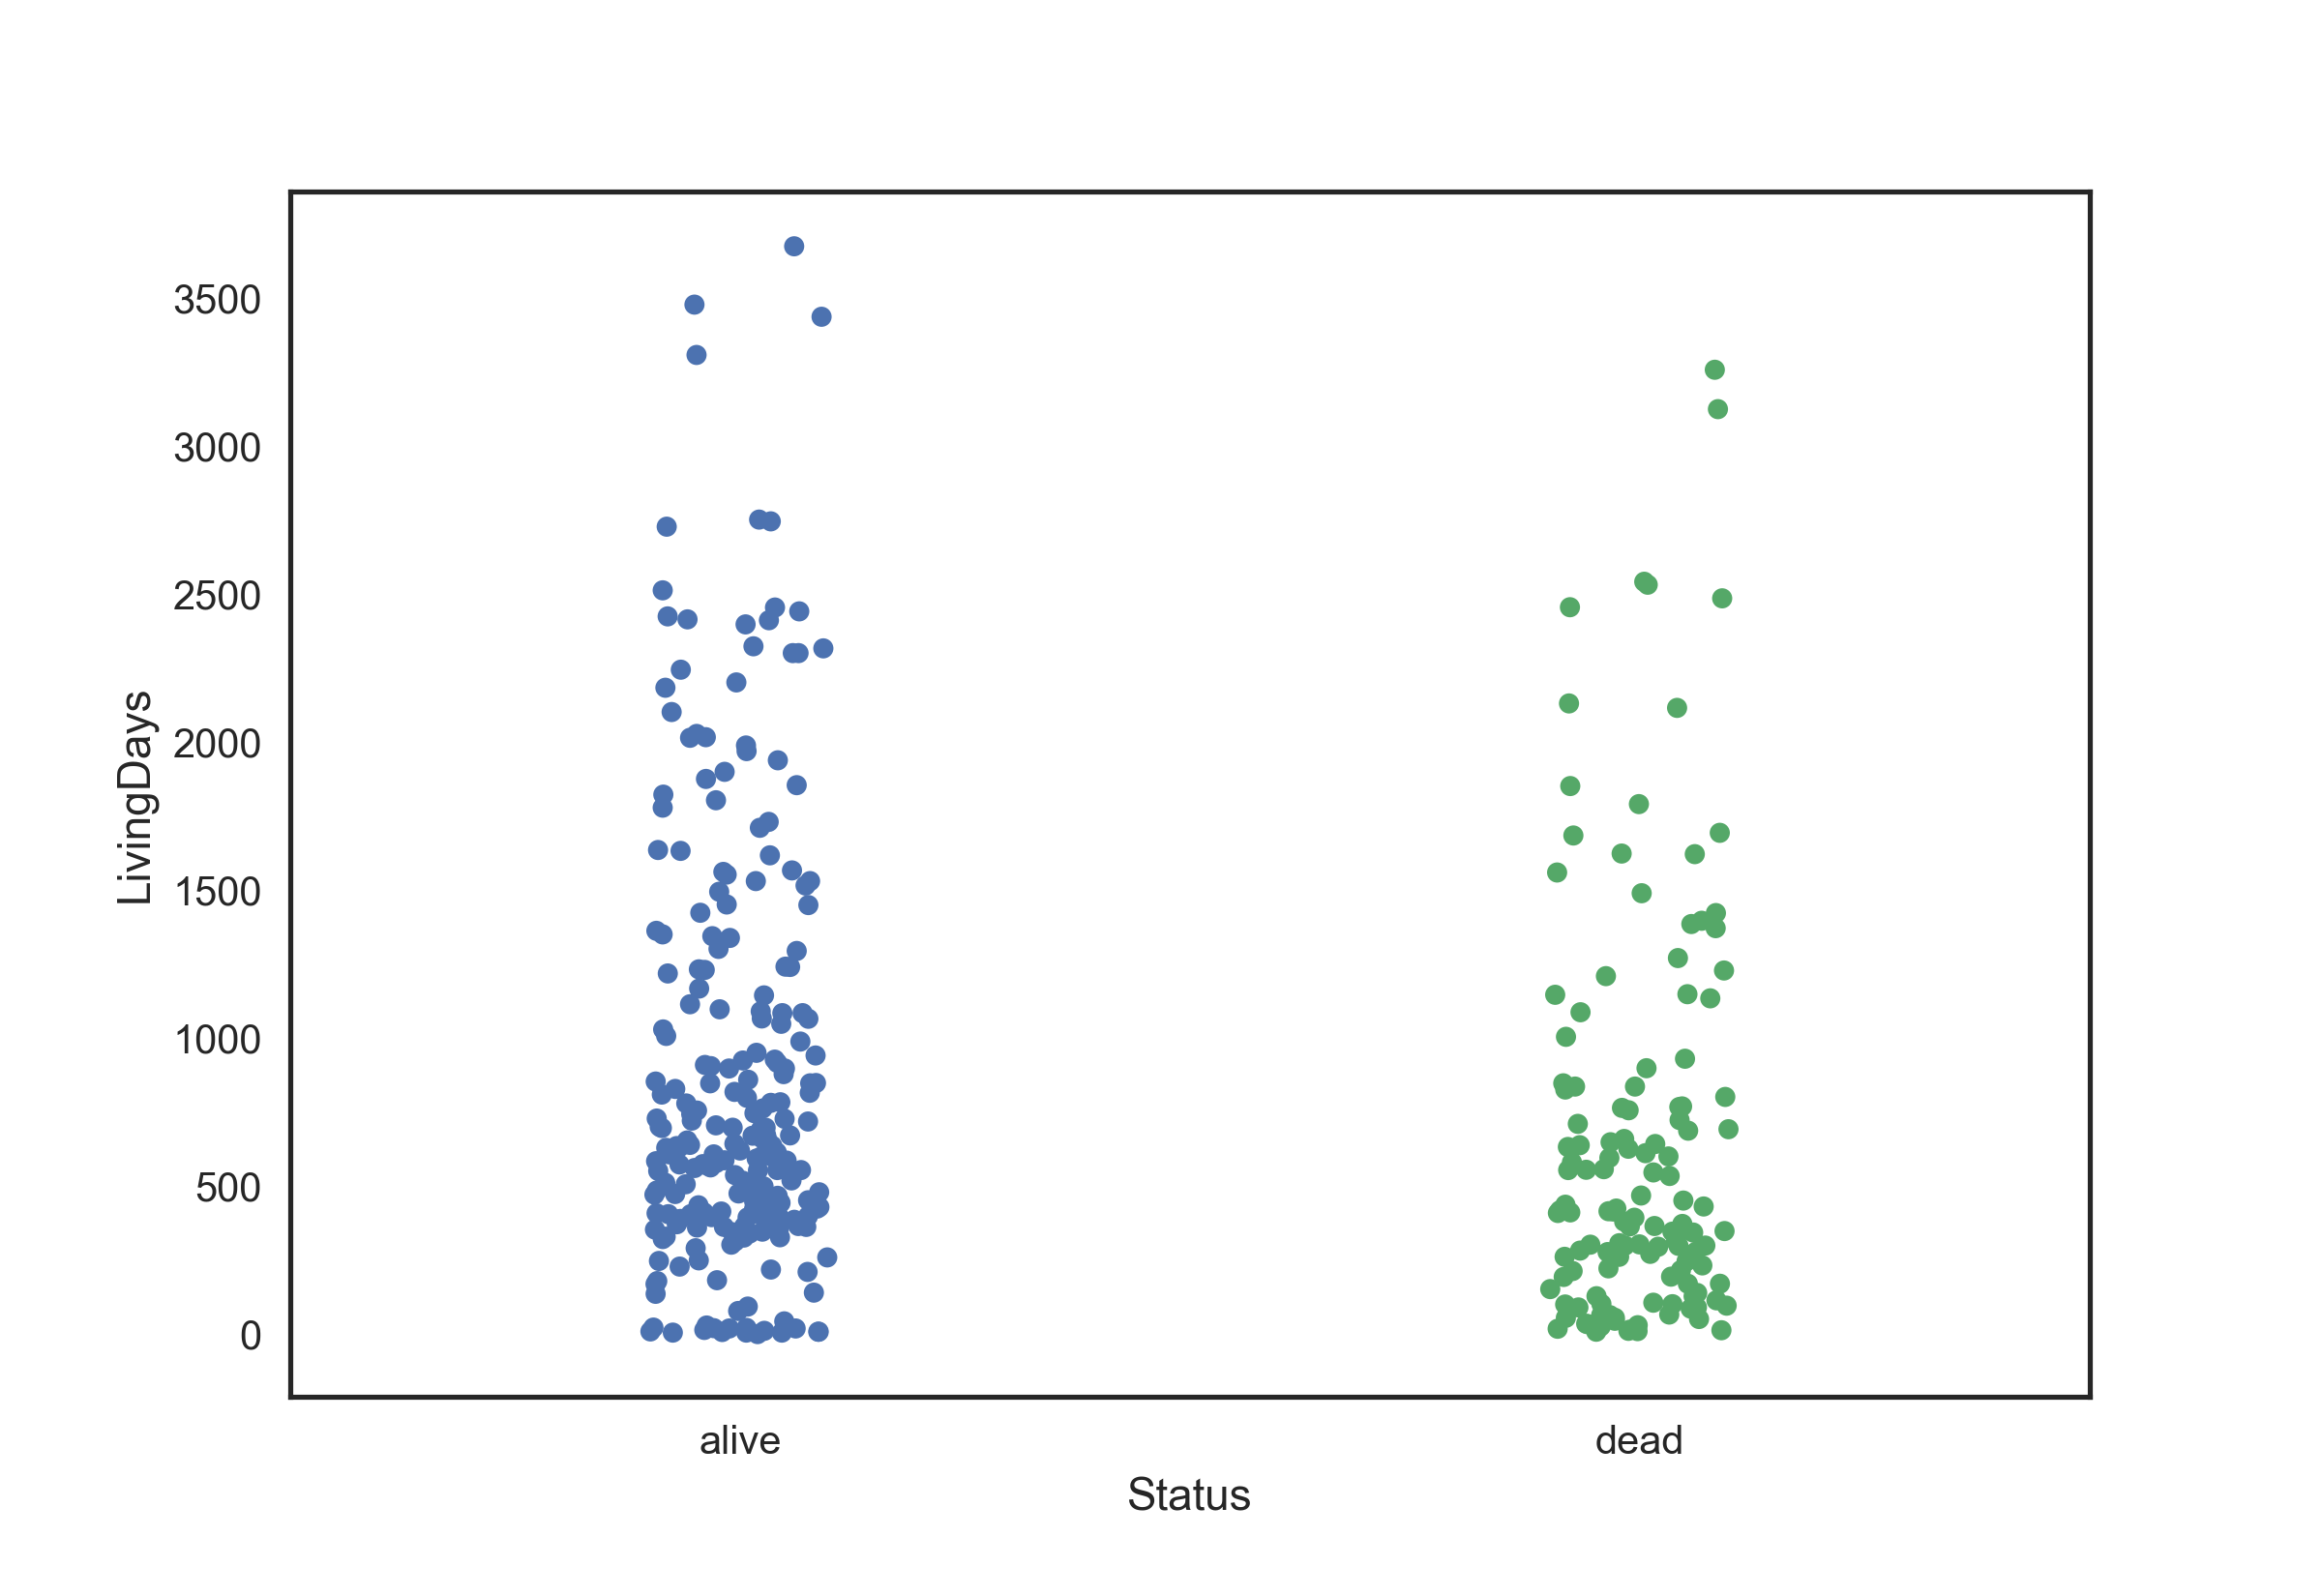
\includegraphics[width=1.1\textwidth]{livingstatusandstatus.png}
        \caption{A gull}
        \label{fig:gull}
    \end{subfigure}
    \begin{subfigure}[h]{0.45\textwidth}
        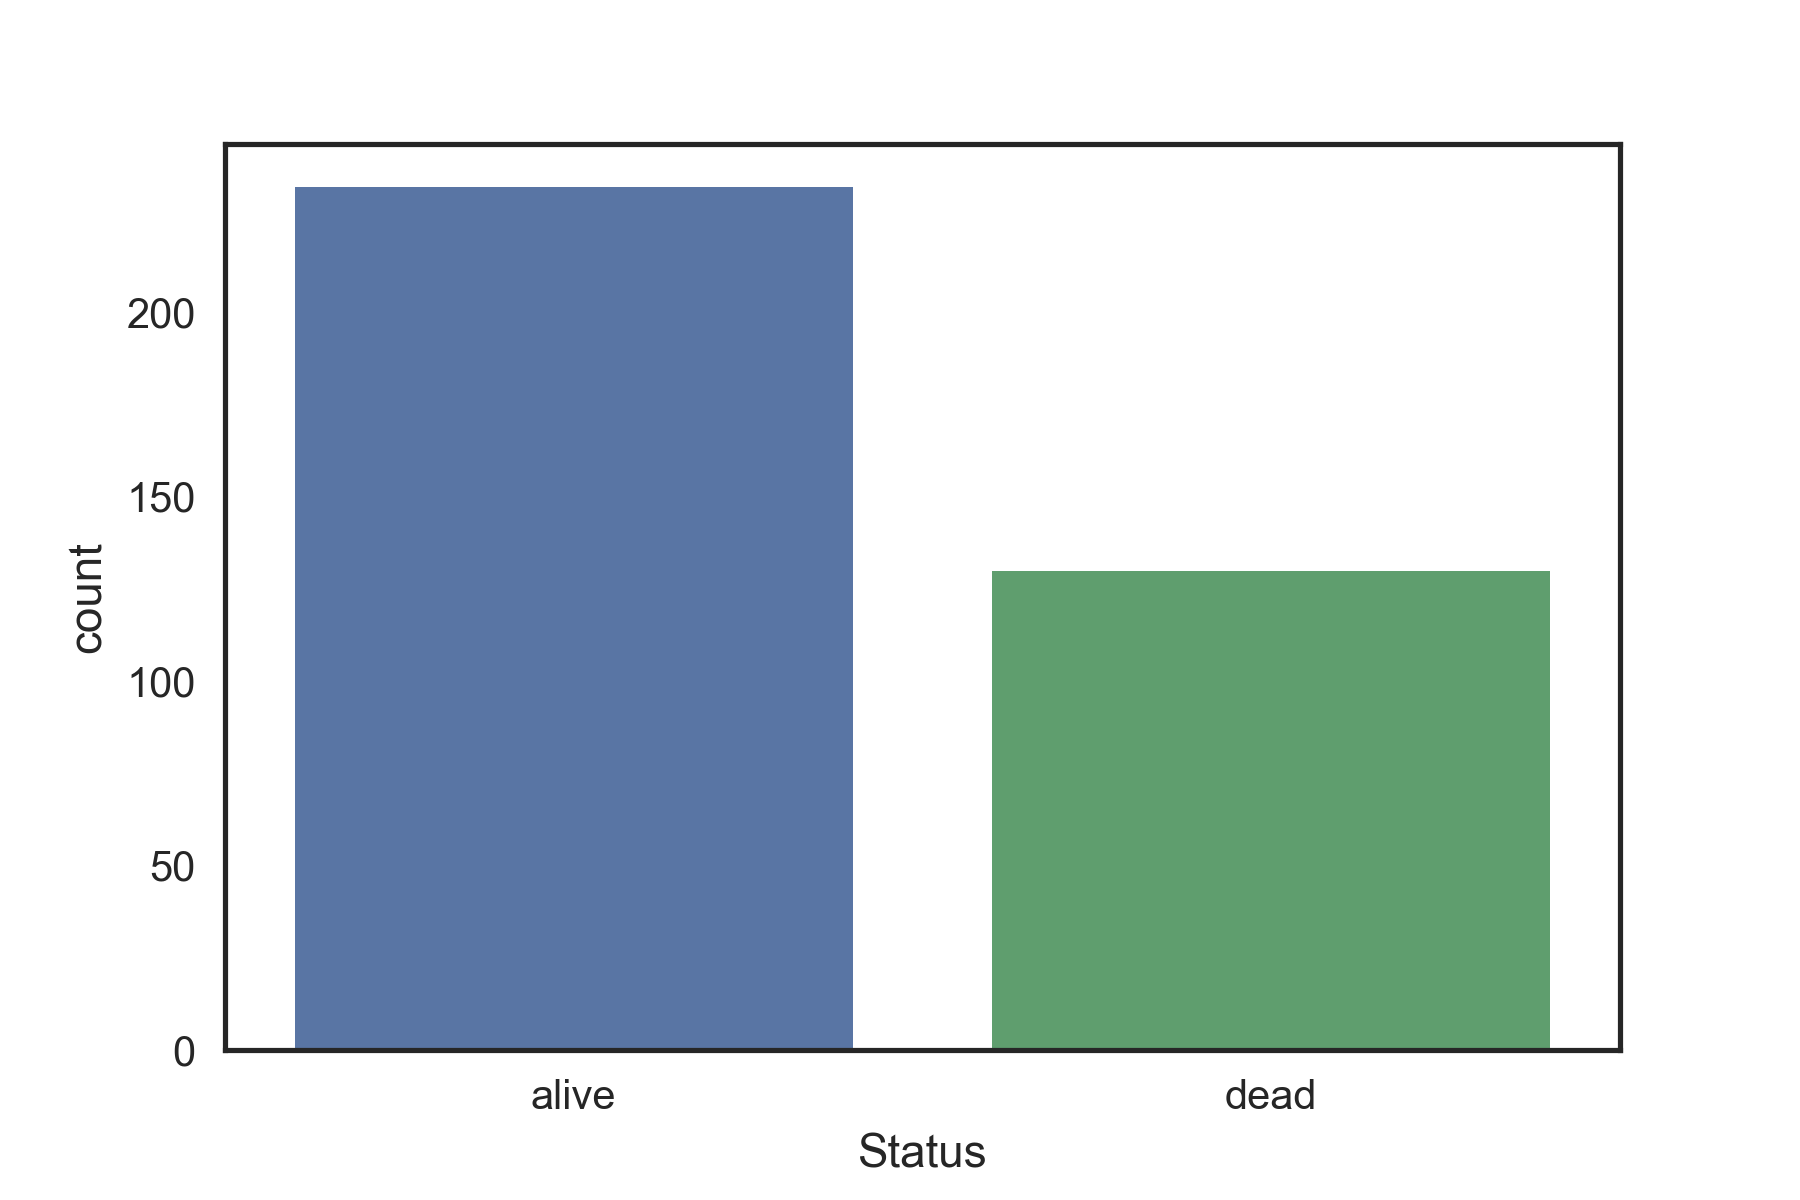
\includegraphics[width=1.1\textwidth]{GenderVSstatus.png}
          \caption{A tiger}
          \label{fig:tiger}
    \end{subfigure}
    \caption{Pictures of animals}\label{fig:animals}
\end{figure}
  

 

 
 \subsection {}
\subsection {}



\bibliographystyle{unsrt}
\bibliography{lib}

\end{document}